\documentclass[12pt]{article}
\usepackage[a4paper, margin=2.5cm]{geometry}
\usepackage{setspace}
\doublespacing

\usepackage{titling}

\usepackage{fancyhdr}
\pagestyle{fancy}
\fancyhf{}
\rfoot{\thepage}
\renewcommand{\headrulewidth}{0pt}

\usepackage{graphicx, tikz}
\usetikzlibrary{automata, positioning, matrix, shapes.geometric, arrows}
\tikzstyle{startstop} = [rectangle, rounded corners, minimum width=3cm, minimum height=1cm,text centered, draw=black, fill=red!30]
\tikzstyle{process} = [rectangle, minimum width=3cm, minimum height=1cm, text centered, draw=black, fill=blue!20]
\tikzstyle{arrow} = [thick,->,>=stealth]

% fix to weird numbering of figs and tables
\renewcommand{\thetable}{\arabic{table}}
\renewcommand{\thefigure}{\arabic{figure}}

\usepackage{parskip, multicol, float}
\usepackage[hidelinks]{hyperref}
\usepackage{amsmath, amssymb}

\usepackage[backend=biber, style=ieee]{biblatex}
\addbibresource{sources.bib}

\usepackage{algpseudocode}

\usepackage[acronym]{glossaries}
\newglossaryentry{stochastic}{
    name=stochastic,
    description={influenced by random behavior}
}

\newglossaryentry{memory depth}{
    name=memory depth,
    description={the length of past outputs in a markov chain that directly influence the outcome of the next output}
}

\newglossaryentry{state}{
    name=state,
    description={a member condition/section within a markov chain that holds distinct weights or rules for producing outputs}
}

\newglossaryentry{output}{
    name=output,
    description={the observed produced result of a markov chain by any singular state}
}

\newglossaryentry{output-specific variance}{
    name=output-specific variance,
    description={a measure of the deviation of a specific output probability from its unbiased equivalent (100\% divided by the number of possible outputs) as the absolute difference between the two}
}

\newglossaryentry{coin-wide variance}{
    name=coin-wide variance,
    description={the sum of the output-specific variances for each output probability within a coin's probability distribution}
}

\newglossaryentry{system-wide variance}{
    name=system-wide variance,
    description={the sum of all coin-wide variances for every coin within a system}
}

\newglossaryentry{probability distribution}{
    name=probability distribution,
    description={the discrete probability density distribution of length $n$ for producing an output $o \in \{0, 1, 2, \dots, n\}$}
}

\newglossaryentry{observed probability distribution}{
    name=observed probability distribution,
    description={the directly observed probability distribution (based on a string of outputs)}
}

\newglossaryentry{hidden probability distribution}{
    name=hidden probability distribution,
    description={the probability distributions held by each coin in the markov chain}
}

\newglossaryentry{standing distribution}{
    name=standing distribution,
    description={the long-term \gls{observed probability distribution} of a markov chain}
}

\newglossaryentry{transition rules}{
    name=transition rules,
    description={a lookup-table of mappings of outputs of size $m$ (\gls{memory depth}) to the next \gls{state}}
}
\makeglossaries

\title{Reverse-Engineering Hidden Markov Models}
\author{Mufaro Machaya and Ian Matsunaga\\Mentor: Brian Marcus, PhD\\Science One, University of British Columbia}
\date{March 2025}

\begin{document}

\pagenumbering{gobble}
\begin{titlepage}
\maketitle
\end{titlepage}
\newpage
\pagenumbering{arabic}

\begin{abstract}
Where conventional models are useful for proportional data, stochastic models are powerful statistical tools for modeling probabilistic data, such as in weather forecasting or epidemic prevention. Research into stochastic modeling largely focuses on the direct applicability of methods for interpreting these models from observed data with less attention given to the reliability and limitations of these models. As such, this study examines the relationship between the complexity of stochastic systems and the error of their reverse-engineering assuming strictly deterministic transition rules are known, allowing for all error to be strictly in the probabilistic deviation of a model's observed probability distribution from its true probabilities. To simulate these systems, models resembling systems of weighted dice were used. An initial or true system was generated at random, a complexity score is calculated from this model based on its weights and memory depth, a chain of 10,000 outputs was produced form this model, a histogram-based algorithm approximated this model using the transition rules, and then the difference these two models' probabilities are used as an error score. This process was repeated 1000 times, and overall, the results showed that increasing this memory depth resulted in a linear or quadratic increase in error, but these increases to memory result in considerably greater increases to maximum complexity with modest increases to maximum error, suggesting that these more complex systems still remain somewhat predictable.
\end{abstract}

\newpage
\section{Introduction}
Markov chains are statistical tools that can be used to describe situations that are stochastic (influenced by random behavior) by modeling how the probability of an event occurring depends on both the specific probability of that event within the context in which the event is occurring and all events that have occurred previously\cite{MARKOVTEXTBOOK}. 

\begin{figure}[H]
\centering
\includegraphics[width=0.5\textwidth]{images/weathermarkov.png}
\caption{An example of the use of a markov chain for describing weather patterns, showing the relationship between each weather outcome\cite{weather-markov-source}.}
\label{fig:weather-markov}
\end{figure}

A common example for the use of a Markov Chain is in describing weather patterns, as the probability of a specific outcome on the weather is heavily influenced by previous weather. For example, the probability of rain is far higher when previous days are either cloudy or rainy, but after numerous successive days of rain, the probability of rain begins to decrease and the probability of other weather outcomes (such as overcast or sunny) begin to increase. In this case, the probability of a specific event is not only dependent on the immediate previous event, but also a series of events up to a reasonable limit, and this depth of outcomes can be said to be the "memory depth" of the system, or how many previous events influence the next output or state that will occur.

The goal of this study is to investigate the relationship the complexity of a stochastic model (markov model) on the accuracy by which that model can be reverse-engineered (measured in error) based on a strictly deterministic reverse-engineering process rather than a traditionally probabilistic one.

\section{Methods}

The Markov chains used in this study are defined as systems resembling the interactions between dice/coins (where each die or coin is a state the system can occupy), where each system has a given size (denoted $n$) describing both the total number of states and outputs each system can produce within the system, a memory depth (denoted $m$), and for every state (coin/die) within the system, a list of transition rules (denoted $T$) mapping a sequence of outputs of length $m$ to the next state and a probability distribution (denoted $P$) describing the probability of producing a given output.

\begin{figure}[H]
\centering
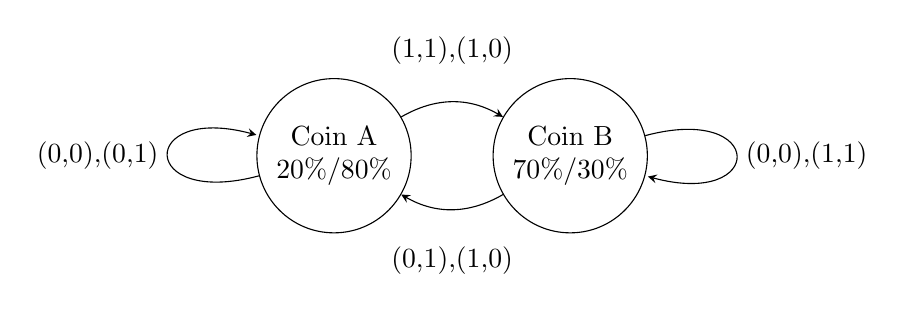
\begin{tikzpicture}[->, >=stealth, node distance=3cm, auto, scale=1, transform shape]

    % Define states
    \node[state, align=center] (A) {Coin A\\20\%/80\%};
    \node[state, right of=A, align=center] (B) {Coin B\\70\%/30\%};

    % Transitions
    \path   (A) edge [loop left]  node              {(0,0),(0,1)} (A)
                edge [bend left]  node[yshift=1em]  {(1,1),(1,0)} (B)
            (B) edge [loop right] node              {(0,0),(1,1)} (B)
                edge [bend left]  node[yshift=-1em] {(0,1),(1,0)} (A);

\end{tikzpicture}
\label{fig:coin-system-example}
\caption{An example of a size $n=2$, memory depth $m=2$ coin system. State/Coin A has probability distribution $P_{A}=(20\%, 80\%)$ and State/Coin B has probability distribution $P_{B} = (70\%,30\%)$ for Heads (0) and Tails (1) respectively. The transition rules $T$ are defined based on every possible combination of all $n$ outputs of length $m$ and unique for each state/coin in the system. For example if the current state was A and the model produced output tails (1), it would check the previous $m$ outputs to decide which state to move to next. As this model is $m=2$, it would also examine the previous output. Suppose that the previous output was also tails (1), the model would use the sequence (1,1) and the transition rules to decide to move to state B. If the next output at state B was heads (0), the model would use the sequence of the previous and current outputs (1,0) to decide to move to state A.}
\end{figure}

For example, a coin system containing two coins with two outputs ($n=2$) with a memory depth of $m=2$ is shown in figure \ref{fig:coin-system-example}, and numerically, it could be represented through the use of a $2 \times 2$ square matrix representing the probabilities and a lookup table for the transition rules.

\begin{table}[H]
\centering
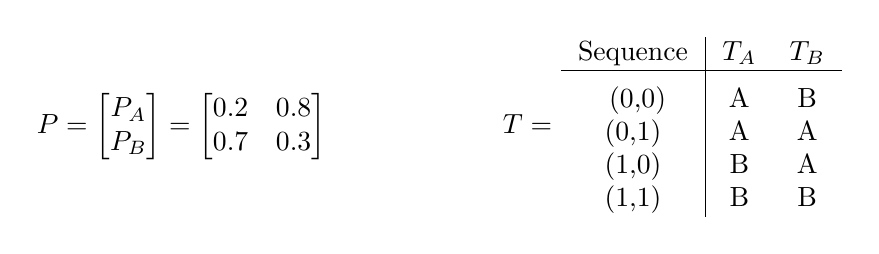
\begin{tikzpicture}

    % Transition Matrix (Left Side)
    \node (T) {$P = \begin{bmatrix} P_A \\ P_B \end{bmatrix} = 
    \begin{bmatrix} 0.2 & 0.8 \\ 0.7 & 0.3 \end{bmatrix}$};

    % Table (Right Side)
    \node (M) [right=2cm of T] {
        $T =$
        \begin{tabular}{c|c c}
            Sequence & $T_{A}$ & $T_{B}$ \\ 
            \hline\rule{0pt}{13pt}
            (0,0) & A & B \\
            (0,1) & A & A \\
            (1,0) & B & A \\
            (1,1) & B & B \\
        \end{tabular}
    };

\end{tikzpicture}
\label{tbl:coin-system-numerical-description}
\caption{A continuation of the example shown in figure \ref{fig:coin-system-example}, displaying the probabilities $P$ as a square matrix of size $n \times n$ and the transition rules as a lookup table mapping a series of outputs $m$ long to the next coin in the chain based on the present coin.}
\end{table}

Commonly, the transition rules between states for a Markov chain is also defined using an $n \times n$ matrix in the form of a transition probability distribution, but in this case, we've opted to define the transition rules as a deterministic lookup-table of mappings of sequences of size $m$ to the next state for each state within the chain rather than a probabilistic form due to the outputs and states under this experiment being distinct (the outputs and states are not the same thing for a die system, but they are for problems like weather modeling), and because this allows for the explicit definition of a memory-depth.

Additionally, in this study, two key statistics are used for analyzing the behavior of these models: complexity and error. Every model has a complexity rating (denoted $c$) defined by the formula
\begin{equation}\label{eq:complexity}
c = nvm^2,
\end{equation}
where $n$ is the size of the model, $m$ is the memory depth, and $v$ is the system-wide variance of the model. The square of the memory is used to emphasize the relative importance of memory as compared to variance and size for a given system. This arbitrary quantification is effective because it is only used to compare with other models with the same measurement of complexity. 

The system-wide variance is defined as the sum of the state-wide variance for a state of the model by equation
\begin{equation}\label{eq:sw-variance}
    v = \sum_{i=1}^{n} Var(S_{i}),
\end{equation}
where $S_{i}$ is state (or die) $i$ in the system, and it's the sum of the output-specific variance of every output on the state's probability distribution.

The output-specific variance is defined as the absolute difference of an output from its expected, unbiased equivalent ($100\%$ divided by the number of outputs), thus state-wide variance is defined as
\begin{equation}\label{eq:ind-variance}
    Var(S) = \sum_{i=1}^{n} |P_{S,i} - \mu|,
\end{equation}
where $P_{S,i}$ is the probability for output $i$ on state $S$, and $\mu = \frac{1}{n}$ is the unbiased probability.

By the law of large numbers, each of these models is guaranteed to converge to a specific standing distribution when run to produce an infinitely long series of outputs\cite{tribello_law_2025}. Any mismatch in the standing distributions of two models guarantees that there is error (or dissimilarity) between the two models, but a match does not guarantee similarity as multiple models with considerably different internal weights can have the same standing distribution. However, in this study, as transition rules are identical between the input and output models, it can be reasonably assumed that the source of error between two models is due to the differences in their respective probability distributions.

As such, we chose to define error as the sum of the absolute differences between their respective output probabilities for every state:
\begin{equation}\label{eq:error}
    E(I,O) = \sum_{i=1}^{n} \sum_{j=1}^{n} |P_{I_{i,j}} - P_{O_{i,j}}|,
\end{equation}
where $I$ is the input model (the "true" model, before reverse-engineering), $O$ is the output model (the reverse-engineered model), $P_{I_{i,j}}$/$P_{O_{i,j}}$ is the probability of producing output $j$ on state $i$ for the input/output model ($I$/$O$).

For each test, we randomly generated 1000 die systems, each with psuedo-random weights (probabilities and transition rules, with all probabilities being normalized such that they add up to 1.0 or $100\%$) within a range of $n \in \{1, 2, 3, 4, 5\}$ and $m \in \{1, 2, 3, 4\}$, with each initially-generated model referred to as the "input model." The input model was then run/flipped to produce a sequential list of outputs $L=10^4$ long. Then, this sequence of outputs and select data about the model is passed into the reverse-engineering algorithm, and the overall testing pipeline is described in figure \ref{fig:core-pipeline}.

\begin{figure}[H]
\centering
\resizebox{0.7\textwidth}{!}{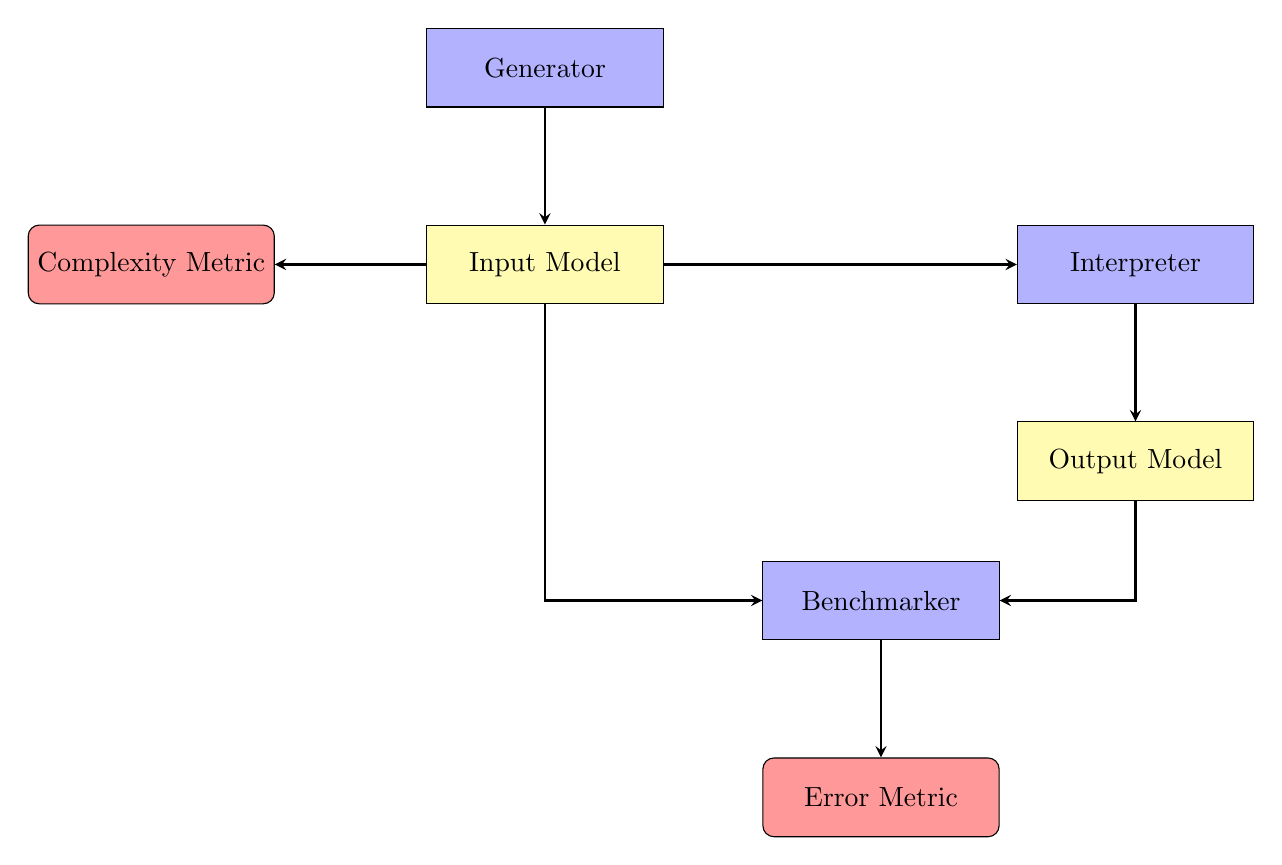
\begin{tikzpicture}[node distance=2.5cm]

    % Nodes
    \node (generator) [process, fill=blue!30] {Generator};
    \node (inputmodel) [process, below of=generator, fill=yellow!30] {Input Model};
    \node (interpreter) [process, right of=inputmodel, xshift=5cm, fill=blue!30] {Interpreter};
    \node (outputmodel) [process, below of=interpreter, fill=yellow!30] {Output Model};
    \node (benchmarker) [process, below right of=inputmodel, xshift=2.5cm, yshift=-2.5cm, fill=blue!30] {Benchmarker};
    \node (error) [startstop, below of=benchmarker, fill=red!40] {Error Metric};
    \node (complexity) [startstop, left of=inputmodel, xshift=-2.5cm, fill=red!40] {Complexity Metric};

    % Arrows
    \draw [arrow] (generator) -- (inputmodel);
    \draw [arrow] (inputmodel) -- (interpreter);
    \draw [arrow] (interpreter) -- (outputmodel);
    \draw [arrow] (inputmodel) |- (benchmarker);
    \draw [arrow] (outputmodel) |- (benchmarker);
    \draw [arrow] (benchmarker) -- (error);
    \draw [arrow] (inputmodel) -- (complexity);

\end{tikzpicture}}
\label{fig:core-pipeline}
\caption{The overall pipeline of the testing process. All generation/processing steps are colored in blue, all models are filled in yellow, and the resultant statistics (complexity and error) are filled in red. In the pipeline, input die systems are generated randomly at the generator, and the complexity for each is immediately calculated. Then, these models are sent into the interpreter and an approximation, the output model, is produced. Lastly, both the input and output models are passed into the benchmarker to calculate the error between them.}
\end{figure}

To reverse-engineer these models, our interpreter uses a simple histogram-based solver that determines the probability distribution by iterating through the outputs, using the transition rules to change between states, and accumulating the history of outputs for each state. Once this process is complete, the history of outputs is divided by the total number of outputs and transformed into probabilities for each state. (see Appendix \ref{appendix:algorithms}). Naturally, this requires prior knowledge of the full transition rules of the system, and as such, its operation relies on the assumption that the transition rules are already known. Knowledge of the transition rules is not necessary to reconstruct the original model from stochastic data, but the lack of it causes the reverse-engineering process becomes too computational complex for the range of this project. 

Once reverse-engineered, the input model is then compared against the output model to generate an error score, and then the error score is graphed against the input model's complexity.

\section{Results}
To begin, the overall trend from testing the data showed a positive/direct relationship between the complexity of a system and its error in being reverse-engineered. 

\begin{figure}[H]
    \centering
    \includegraphics[width=0.5\textwidth]{images/graph-all.png}
    \caption{All of the data from randomly generating 1000 die systems between the sizes of 1 to 5 and memory depths of 1 to 4, with each data point color coded by the memory depth of its input model. Distinct patterns are visible for each memory depth, with higher memory depths associated with larger relative error ranges. }
    \label{fig:all-data}
\end{figure}

To further investigate this trend, this data can be split into respective graphs for each memory depth.

\begin{figure}[H]
    \centering
    \includegraphics[width=0.35\textwidth]{images/graph-mem1.png}
    \includegraphics[width=0.35\textwidth]{images/graph-mem2.png}
    \includegraphics[width=0.35\textwidth]{images/graph-mem3.png}
    \includegraphics[width=0.35\textwidth]{images/graph-mem4.png}
    \caption{The data from \ref{fig:all-data} split into each of the respective memory. Both linear and quadratic fits have been applied, with relatively equal level of fitting (as shown with $R^{2} \approx 0.88-0.90$ for all fits), so a strong conclusion cannot be drawn for the type of positive relationship between complexity and error. Interestingly, the linear slopes ($k$) decrease given increase to memory, as $m=1$ has $k \approx 3.1$ and $m=4$ has $k \approx 1.2$.}
    \label{fig:data-split}
\end{figure}

\section{Discussion}

As shown in figure \ref{fig:all-data}, a higher memory depth does not necessarily seem to result in a higher error, but a higher complexity generally seems to result in a higher error in a somewhat linear relationship, as there is a comparably low error at low complexities compared to higher complexities.

As expected, an overall direct, positive trend between the complexity of a system and the error in reverse-engineering it was observed. However the memory depth plays the most dramatic role in determining the rate at which the error of the system increases, as variance and size increases. The trends seen in figures \ref{fig:all-data} and \ref{fig:data-split} show that for each memory depth, there is a distinct slope as the models within that memory depth increase in complexity, indicating that the error increases locally for each memory depth.

Each memory depth clearly has an associated maximum complexity for any generated model of that depth, due to the maximum size models can be generated at, and an innate max variance any model can have for any size. Analyzing each memory's range of complexity shows that as memory increases, the range of complexity increases relatively linearly. However, the range of error for each memory appears to increase less for each jump between memory. This may potentially be due to a limit to the maximum error any reverse engineered model can have, and so as the memory depth increases the associated range of error begins to increase at a slower rate due to approaching this limit. Since each memory depth has a generally direct, positive linear relationship between complexity and error this leads to a decreasing slope as memory depth increases. 

Given that the interpreter algorithm operates on already knowing the full set of transition rules and building a histogram for each output on every state, this system should theoretically result in little to no error for every stochastic system, so the source of the error being witnessed (and its increase in magnitude alongside an increase in complexity) could be due to some fundamental misalignment of the algorithm. However, most likely, the source of the error is due to the dataset not being long enough for the overall distribution of outputs to be fully converged to the stationary distribution of the input model. If the dataset is not sufficiently large, unavoidable random variation in the outputs will still remain significant and therefore affect the reverse-engineering process.

\section{Conclusion}
The relationship between complexity and error was determined to be directly positive, with the trend for increase being distinct for each memory depth value and roughly quadratic with respect to the size of the system. When reverse-engineering non-randomly generated data (e.g., real world weather data) we found that when more complex models best approximated the patterns in the data, they were associated with higher error, similarly illustrating the validity of the findings with generated data.

\section*{Data Availability Statement}

As of March 2025, all of the source code and analysis data are publicly available in the GitHub repository \texttt{nickelulz/sci1-term-2}\cite{source-repository}. For algorithm pseudocode, see \ref{appendix:algorithms}.

\printbibliography

\appendix

\newpage
{
\onehalfspacing
\section{Reverse Engineering Algorithm}\label{appendix:algorithms}
\begin{algorithmic}
\Procedure{Reverse-Engineer}{sequence, $n$, $m$, $T$}
    \State coins/outputs \textbf{is} $\{0, 1, 2, \dots, n\}$
    \State histogram \textbf{is} $n \times n$ matrix of zeroes
    \State memory \textbf{is} empty list
    \State current-coin \textbf{is} $S_0$ \\

    \Comment{\parbox{0.7\linewidth}{\textit{Iterate through the output sequence and follow the transitions using the transition matrix to build a histogram counting the number of times each coin generated a specific output.}}}

    \ForAll{output \textbf{in} sequence}
        \State histogram(current-coin, output) $\mathrel{+{=}} 1$
        \State \textbf{append} output \textbf{to} memory \\
        
        \If{\textbf{length of} memory \textbf{equals} $m$}
            \State current-coin \textbf{is} $T$(current-coin, memory)
            \State \textbf{clear} memory
        \EndIf
    \EndFor

    \Comment{\parbox{0.7\linewidth}{\textit{Convert the list of histograms into individual probability distributions for each coin by calculating a sum of outputs for each coin and dividing the count for a given output by the output sum for that coin.}}}

    \State probabilities \textbf{is} $n \times n$ matrix of zeroes
    
    \ForAll{coin \textbf{in} coins}
        \State total $:=$ 0
        \ForAll{ouput \textbf{in} outputs}
            \State total $\mathrel{+{=}}$ histogram(coin, output)
        \EndFor
        \ForAll{output \textbf{in} outputs}
            \State probabilities(coin, output) = histogram(coin, output) / total
        \EndFor
    \EndFor 
    
    \State \Return \textbf{new coin with} probabilities, $T$
\EndProcedure
\end{algorithmic}
}

\end{document}
